\section{Materiais e Métodos}

%----------------------------------------------------
\begin{frame}{Seleção de Critérios}

\begin{figure}[!h]  
		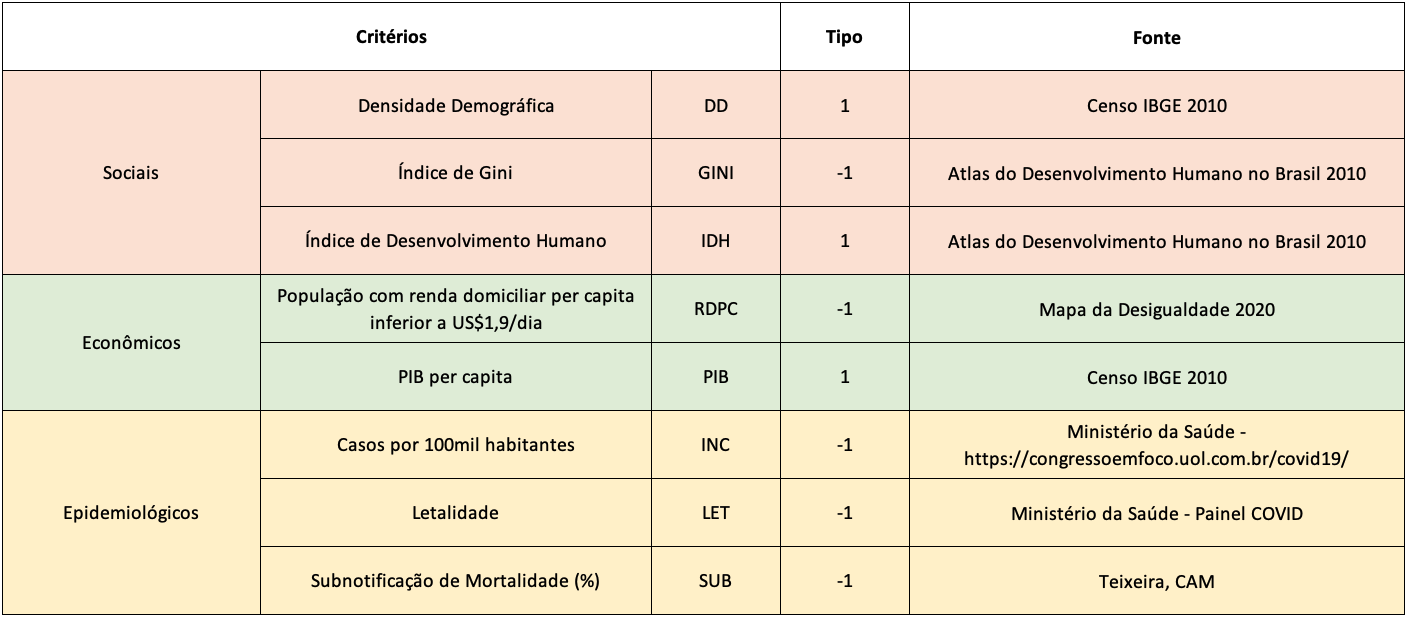
\includegraphics[width=.9\textwidth]{figs/criterios}
	    \label{fig:criterios}
\end{figure}
	
\end{frame}

%----------------------------------------------------
\begin{frame}{Definição de Pesos}

Pesos definidos por dois métodos distintos:

\begin{table}[]
\caption{Definição dos pesos para cada critério}
\label{tab:pesos}
\resizebox{.8\textwidth}{!}{%
\begin{tabular}{@{}lllllllll@{}}
\toprule
\textbf{Método de Definição} & \textbf{DD} & \textbf{GINI} & \textbf{IDH} & \textbf{RDPC} & \textbf{PIB} & \textbf{INC} & \textbf{LET} & \textbf{SUB} \\ \midrule
\textbf{Pesos Iguais}        & 0.125       & 0.125         & 0.125        & 0.125         & 0.125        & 0.125        & 0.125        & 0.125        \\
\textbf{Entropia}       & 0.3764      & 0.0014        & 0.0007       & 0.0838        & 0.0368       & 0.0406       & 0.036        & 0.04244      \\ \bottomrule
\end{tabular}%
}
\end{table}
	
\end{frame}

%----------------------------------------------------
\begin{frame}{Método PROMETHEE II}

\textit{Preference Ranking Organization Method for Enrichment Evaluations II}

\begin{itemize}
	\item Comparação par-a-par de possíveis decisões;
	\item Possíveis decisões são avaliadas de acordo com diferentes critérios (minimização ou maximização)
	\item Pesos e Função de Preferência
\end{itemize}

\end{frame}

%----------------------------------------------------
\begin{frame}{Método PROMETHEE II}

O processo de tomada de decisão consiste em 5 etapas:

\begin{figure}[!h]  
		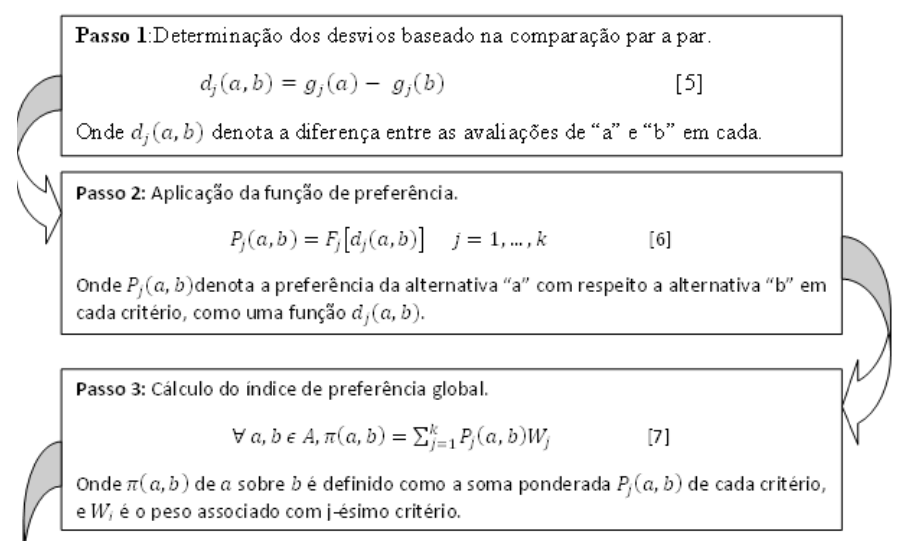
\includegraphics[width=.8\textwidth]{figs/promethee2-1}
	    \label{fig:criterios}
\end{figure}

\end{frame}

%----------------------------------------------------
\begin{frame}{Método PROMETHEE II}

O processo de tomada de decisão consiste em 5 etapas:

\begin{figure}[!h]  
		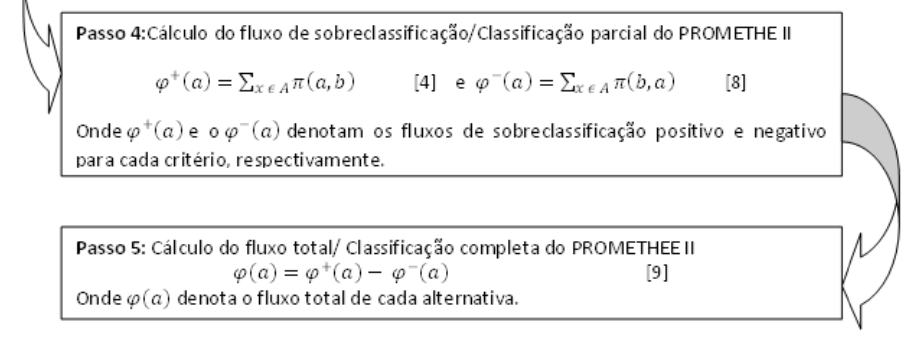
\includegraphics[width=.8\textwidth]{figs/promethee2-2}
	    \label{fig:criterios}
\end{figure}

\end{frame}